\chapter{Fault Attacks}\label{cha:c9_ninthchapter}

\begin{centering}
	\section*{Topics}\label{sec:topics}
		\begin{enumerate}
			\begin{centering}
				\item Introduction to Fault Attacks
				\item Fault Attack on RSA-CRT
				\item DRAM and Rowhammer
				\item Flip-Feng-Shui: Rowhammer attack on RSA \\
			\end{centering}
		\end{enumerate}
\end{centering}
\newpage

\section*{Introduction to Fault Attacks}\label{sec:introduction_to_fault_attacks}
Up until now in the course we learned about \emph{passive} attacks -- i.e.\
attacks which measure \emph{leakage} such as timing information and power
traces. The advantage of these attacks is that they allow an attacker to acquire
information in the process of an ongoing computation e.g.\ an AES key
\emph{before} it was fully mixed with the input -- this fact can help the
attacker extract secrets.

In fault attacks we will become \emph{active} in the sense that we will give the
device-under-test (DUT) additional inputs such as heat or radiation.

One problem with Fault attacks: they use the strongest attack model, meaning --
we assume most power on the attacker's part.

\section{Active Attacks}\label{sec:active_attacks}
\paragraph{Definition:}
\begin{quote}
	\textit{``A faul attack is an active attack that allows extraction of secret information from cryptographic devices by breaking those devices.''}
\end{quote}

In fault attacks we are being \emph{active} -- we give additional inputs beside
the main input such as:
\begin{enumerate}
	\item Fuzzing (garbage or bad input)
	\item Radiation
	\item Heat
	\item Vibration
	\item Power spikes etc.
\end{enumerate}

This way, we receive other (usually erroneous) outputs which might give us
additional information about the computation and/or the secret. This process is
described in \Cref{fig:fault_attacks_schematic}.

\begin{figure}[!ht]
	\centering
	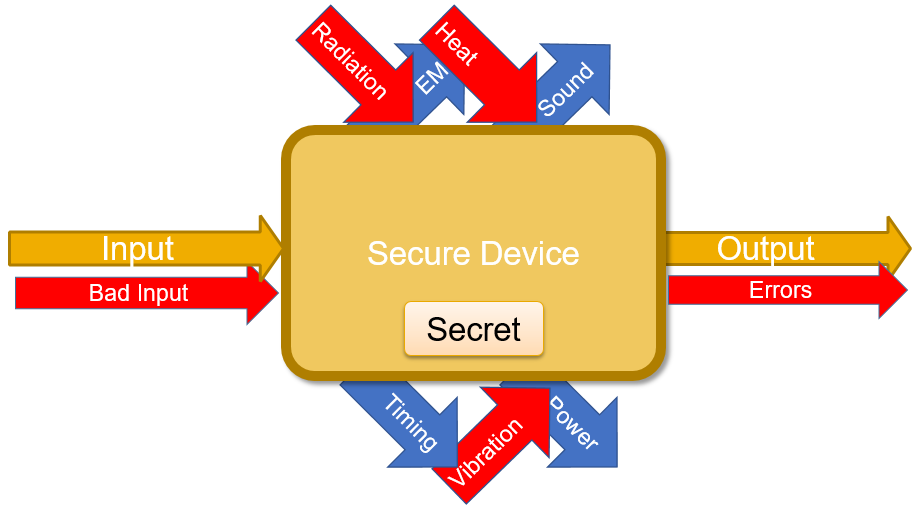
\includegraphics[width=0.7\linewidth]{images/chapter_9/fault_attacks_schematic.png}
	\caption{A schematic diagram of fault attacks and leakage types.}\label{fig:fault_attacks_schematic}
\end{figure}

Like with passive attacks, some of those outputs can be acquired at different
stages of the computation process.

Many fault attacks are inspired by studies in the field of \emph{reliability}: a
study in reliability will research a device's physical boundaries e.g.\ the
maximum or minimum temperature under which it performs reliably. Other examples
of reliability studies are aimed at improving device performance under extreme
conditions such as:
\begin{itemize}
	\item Space and X-Rays
	\item Dense CPU Layouts
	\item Data Center Recovery (ECC-RAM)
\end{itemize}

A security researcher implementing fault attacks will, on the other hand,
purposefully subject the DUT to extreme conditions in order to inject errors in
the device's functionality to achieve their goal. In that sense, a reliability
study of a given device can lay the ground-work for the fault attacks to come.

\begin{quote}
	\textit{``In the reliability community things happen by mistake. In the security community -- things happen on purpose.''}
\end{quote}

\subsection*{Breaking a device-under-test}\label{subsec:breaking_a_device_under_test}
How can \emph{breaking} a device help an attacker?

\begin{enumerate}
	\item BORE -- \textit{``Break Once, Run Everywhere''}: Some device families
	share a single secret among all instances.
	\item Repairable Devices: Temporary breakage is fine. Sometimes restarting
	the device is enough to ``repair'' the damage.
	\item Partial breakage: Sometimes it's convenient to break \emph{part} of a
	device, for example -- destroy the subsystem responsible for DRM
	verification.
\end{enumerate}

\section{Fault Attack Taxonomy}\label{sec:fault_attack_taxonomy}
The tree ways we can examine a Fault Attack in order to understand it are:
\begin{enumerate}
	\item Method - \emph{``How to inject?''}
	\item Properties - \emph{``What fault to create?''}
	\item Target - \emph{``Which part to break?''}
\end{enumerate}

\subsection{Fault Methods}\label{subsec:fault_methods}

\subsubsection{Power Supply Attacks}\label{subsubsec:power_supply_attacks}
What happens if the device is underpowered? As we have previously seen, power in
electronic devices is used to drive the CMOS transistors. If the device is
slightly underpowered it might fail to switch some of the transistors and thus
produce false calculations, and with even less power it might  struggle with
getting into operational state (boot loop) or even transition to an entirely
faulty state. Another attack method involving the power supply is injecting
power spikes (to a similar effect).

Some parts of a device are typically more sensitive to the power supply than
others, and thus under- or over-powering the device will de-stabilize it and
inject faults.

The obvious scenario for such an attack is when the DUT belongs to or is being
controlled by the attacker -- for example if they're examining their own set-top
box etc. In that case, the attacker can supply the device with as much/little
power as they wish.

Another example of such attack scenarios is in the field of RFID readers -- the
device powering an RFID chip is the reader, so a \emph{malicious} RFID reader
can over/under-power the chip to achieve various faulty results.

\subsubsection{Clock/Timing Attacks}\label{subsubsec:clock_timing_attacks}
The clock is typically a bus shared by many of the system's components which
synchronizes the propagation of calculations through the system -- i.e.\ at the
beginning all inputs are ready, and when there is a rising edge on the clock bus
they start propagating throughout the various computational components. When all
computations are finished they all wait for the next rising edge on the clock
bus in order to proceed to the next stage. In a clock glitching attack the
attacker would inject a rising edge on the clock bus at an arbitrary time. This
way only \emph{some} of the computations will have finished by that time while
others are still being processed, and thus the device will be in a faulty
(unstable) state.

A notable example is the attack on Mifare Classic RFID chips we talked about in
the beginning of the course~\cite{nohl2008} -- the RNG in the chip is only
dependent on the time between powering up the RFID tag and challenging it. An
RFID reader operated by the attacker can control both parameters, thus making
the generated challenges deterministic.

\subsubsection{Temperature attacks}\label{subsubsec:temperature_attacks}
This attack method relies on the physical property of electrons (current).
Electrons ``jump'', and the higher the temperature -- they will jump more
frequently and to longer distances. If a device gets \emph{too hot} -- enough
electrons can ``jump'' e.g.\ over the insulation layer in a transistor to flip
it from logical 1 to 0. This results in a fault.

Because of the ubiquity of devices failures due to temperature, nowadays
temperature sensors are integrated into most devices, so when it overheats --
the device will shut down.

An attacker can bypass the temperature sensor by disconnecting it. Another
method would be to quickly alternate the temperature of the device from
extremely high to extremely low, so that \emph{on average} the temperature is
reasonable, but it will still experience faults during the extreme phases of the
cycles.

In an interesting research paper~\cite{appel} a type-confusion attack on the
Java virtual-machine was demonstrated: at first, the entire memory was filled
with small arrays (say of size one). The Java VM is type-safe, so it is normally
impossible to access one of the memory regions using a pointer to a different
region. To inject a type-confusion fault the researchers used a 50W light bulb
to heat the memory chip of the device enough to flip some of the bits (for
illustration see \Cref{fig:memory_lightbulb}). As a result, a small portion of
the data-structures describing the arrays in memory now held wrong values (e.g.\
changed their value from \(size=1\) to \(size=20\)). At this point, some
affected data-structure \emph{contains} a header of a different data-structure,
to which the attackers now have read and write access. Changing the header of
the second data structure to an arbitrary value gave the attackers access to the
entirety of the device's memory.

\begin{figure}[!ht]
	\centering
	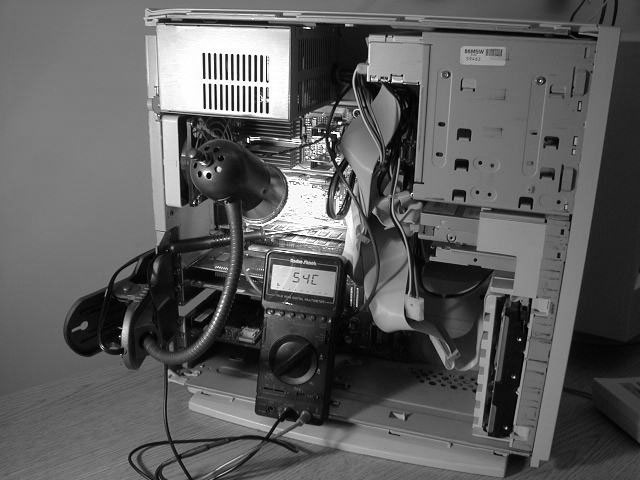
\includegraphics[width=0.7\linewidth]{images/chapter_9/bulb.png}
	\caption{A light bulb flipping memory bits filled with safe Java structures.}\label{fig:memory_lightbulb}
\end{figure}

\subsubsection{Optical, Electromagnetic}\label{subsubsec:optical_electromagnetic}
When a laser hits a transistor it changes the energy level of the silicon
inside, and sometimes it can change the transistor's state. Notably different
wavelengths are absorbed by different materials, so in a typical silicon chip
different lasers will hit different layers of the device etc.
Magnetic/Electromagnetic radiation and pulses have similar effects.

The underlying principal of those attacks is that the attacker forcefully
injects charge (energy) into the device. Once it's stored inside it will have to
dissipate one way or another, so as a result it injects a random faulty state
into the device.

\subsubsection{Reading from RAM}\label{subsubsec:reading_from_ram}
All of the attacks described above require very high engagement with the DUT --
in order for the attacker to control the power/clock sources, for example, they
sometimes would need to drill, cut or otherwise tamper with the device. Shining
a laser on a device requires at the very least having it at a visible distance.

The final attack method involves only \emph{reading} from memory, and thus is
very practical and requires very little physical engagement. This attack method
is called \emph{Rowhammer} and is discussed later in the lecture.


\subsection{Fault Properties}\label{subsec:fault_properties}
In this section we discuss:
\begin{enumerate}
	\item How controllable is the fault's location/size? Precise? Loose? None?
	\item How controllable is the fault timing?
	% Can we have the fault occur when something exciting is happening? Heat is
	% the LEAST controllable -- it's a gradual and stochastic process. Freaking
	% Lasers -- very controllable.
	\item What's the fault's duration? Transient? Permanent? Destructive?
\end{enumerate}


\subsubsection*{Destructive fault attacks on cryptographic devices}\label{subsubsec:destructive_fault_attacks_on_cryptographic_devices}
What can be done with fault attacks to symmetric ciphers? \paragraph{Easy
example:} Imagine that we have a pile of cipher devices with a 64bit key length,
which work the following way: we can give the device a key and it tells us
whether it's the right key.

What if we have a DESTRUCTIVE fault attack that resets the top 32bits of a
device's key? We can brute force the key in \(2\cdot 2^{31}\) instead of
\(2^{63}\) (on average):

First we inject the fault into one of the devices and brute-force the lower 32
bits of the key (\(O(2^{31})\)), then we pick another device from the pile and
brute-force only the higher 32 bits (another \(O(2^{31})\)).

\paragraph{A less trivial example:} We have a public-key device which we can ZAP
and one bit of the key flips to zero.

We can save all of the plaintexts-cipher pairs until we reach the one matching
an all zero key -- which we can pre-calculate. This gives us the Hamming weight
of the key. Now we go back one plaintext-cipher pair -- we know that pair's
key's Hamming weight to be exactly one -- meaning we need to brute-force only
\(N\) keys (\(N\) is the key bit-length). Now we have the position of a single
bit of the key.

If we iterate all the way backwards to the original plaintext-cipher pair, we
can acquire the key in \(O(N^2)\) time!

\subsection{Fault Target}\label{subsec:fault_targets}
What could be targeted by a fault attack?
\begin{enumerate}
	\item Input parameters (fuzzing, clock glitching)
	\item Storage (volatile/non-volatile)
	\begin{enumerate}
		\item HDD -- Destructive (persists after reset)
		\item RAM -- Permanent
		\item Cache -- Transient
	\end{enumerate}
	% If we fault the disk/flash? It's a destructive fault! If we fault the RAM,
	% the fault is permanent (not destructive). In cache? Transient fault! What
	% other storage is there? Instruction cache.
	\item Data processing: inject a fault mid-computation and the device gives a
	different answer.
	\item Instruction Processing/Control Flow: inject a fault in the IP register
	and change the instruction flow.
	\begin{enumerate}
		\item ARM32 instructions are very densely packed, thus there is a very
		high probability of hitting a valid instruction after flipping a single
		bit. \texttt{jnz} and \texttt{jmp} are only one bit apart.
		\item Change for loop condition to dump RAM contents including source
		code.
	\end{enumerate}
\end{enumerate}

\paragraph{Two examples of Fault Attacks targeting Control Flow:}
\begin{enumerate}
	\item The CHDK hacking community, used to dump the firmwares of Canon
	cameras via blinking one of their LEDs~\cite{chdk, canon}.

	\item ``The Unlooper'': Back in the 90's pay-tv devices started
	cryptographically signing the content, and if the cryptographic checksum did
	not check out -- the device would enter an endless loop. The hacking
	community invented ``unloopers'' -- a gadget that would inject a power spike
	and fault the IP register, so that the pay-tv device would jump to some
	other section of the code, from which point it would function normally.
\end{enumerate}

\section{Fault attack on RSA-CRT}\label{sec:fault_attack_on_rsa_crt}

\subsection{RSA decryption}\label{subsec:rsa_decryption}
\(N = p\cdot q\) \(M = C^d \pmod{n} = M^{ed} \pmod{n} = M^1 \pmod{n}\)

RSA decryption is hard!

Let's speed it up using CRT (the Chinese Remainder Theorem): Multiplication
operations are \(O(|n|^2)\). If we can do operations \(\pmod{p}\) and then
\(\pmod{q}\) instead of \(\pmod{n}\), we will reduce computation time by half.

\paragraph{Explanation:}

The bit-lengths of \(p\) and \(q\) are each half that of \(n\)
\[|p|=|q|=\frac{1}{2}|n|\] The computational complexity of multiplying by a
number of length \(x\) is (roughly) \(O(x^2)\). Thus:
\[
O(|p|^2) = O(|q|^2) = \frac{1}{4}O(|n|^2) \Rightarrow (O(|p|^2) + O(|q|^2)) = \frac{1}{2}O(|n|^2)
\]

So if we could multiply by \(p\) and \(q\) instead of by \(n\), we would cut
\emph{each} multiplication operation's time complexity in half!

\subsubsection{Chinese Remainder Theorem}\label{subsubsec:chinese_remainder_theorem}
\begin{figure}[!ht]
	\centering
	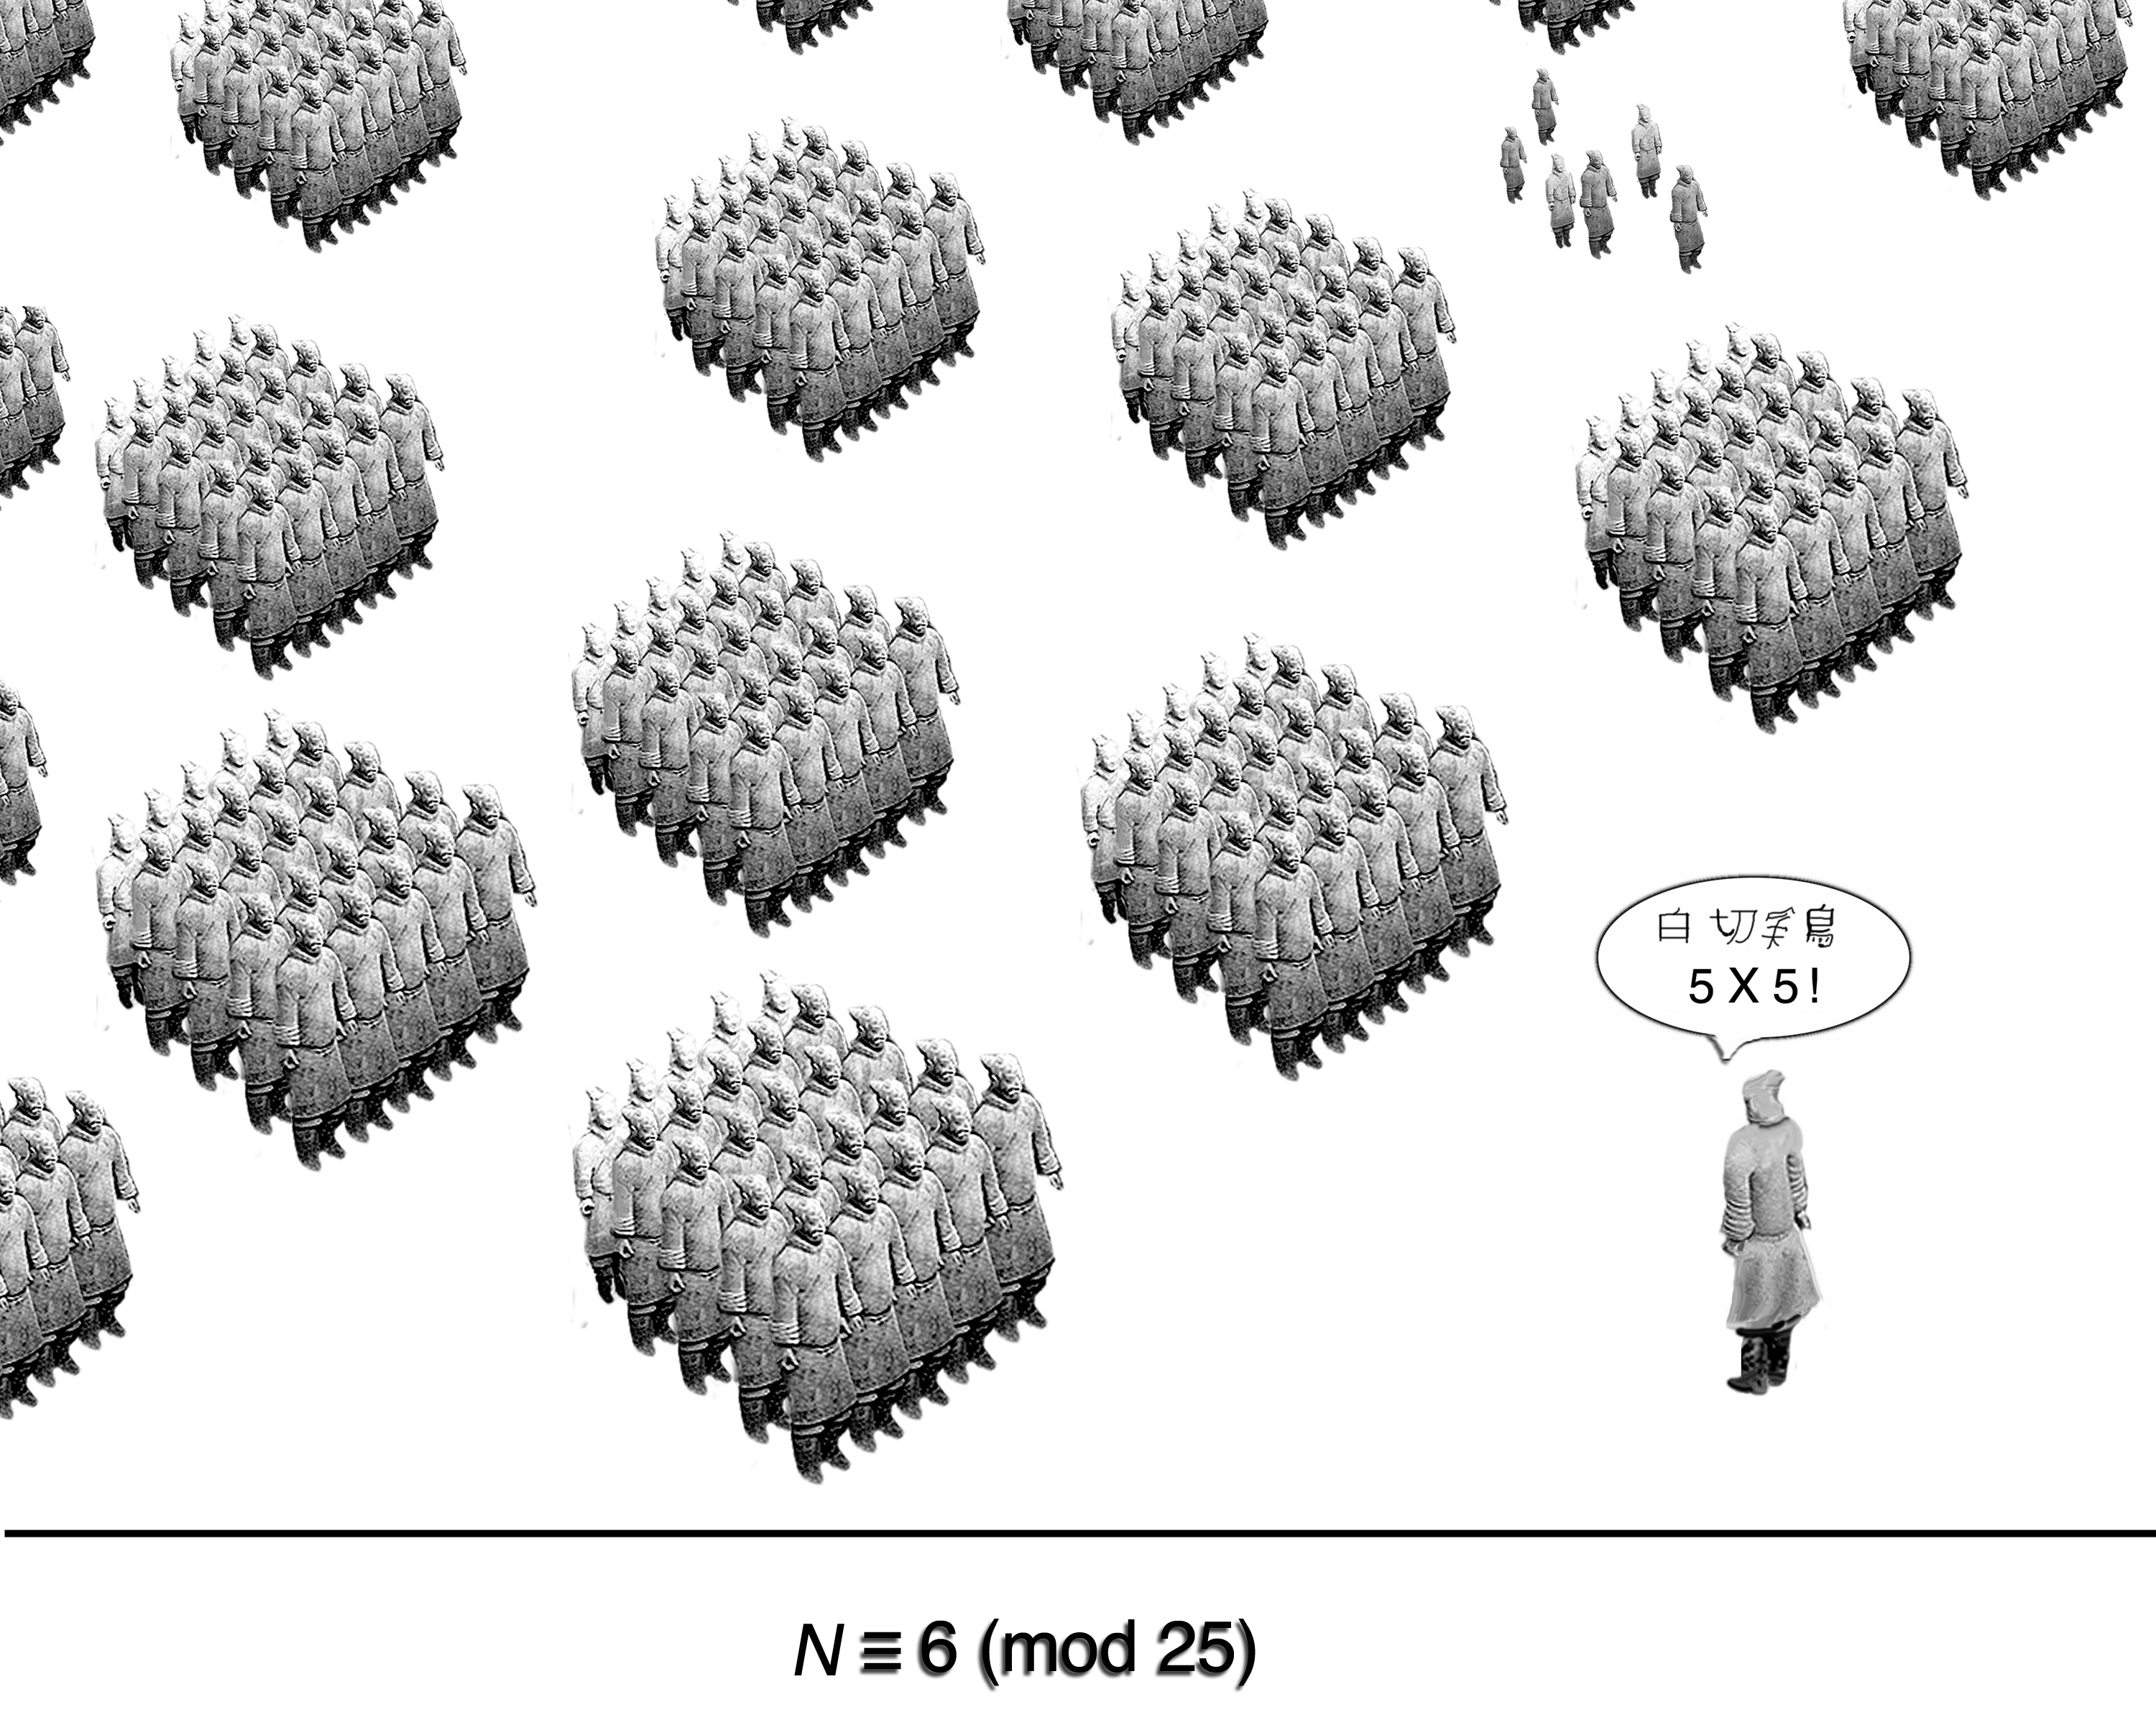
\includegraphics[width=0.5\linewidth]{images/chapter_9/soldiers.jpeg}
	\caption{Chinese Remainder Theorem (Source: \url{https://russinoff.com/papers/crt.html})}\label{fig:chinese_remainder}
\end{figure}
The idea is that if we know both \(x \pmod{p}\) and \(x \pmod{q}\) then we can
easily calculate \(x \pmod{n}\).

So, given a message \(M\) calculate \(M_p\) and \(M_q\): \(M_p = C^d
\pmod{n}\pmod{p} = C^d \pmod{p}\) \(M_q = C^d \pmod{n}\pmod{q} = C^d \pmod{q}\)

To combine the values, we do:
\[M^* = CRT(M_p, M_q) = \]
\[M_p \cdot q \cdot (q^{-1} \pmod p) + M_q \cdot p \cdot (p^{-1} \pmod q)\]

It is easily provable that \(M^* \pmod{p} = M_q\) and \(M^* \pmod{q} = M_p\), so
by the Chinese Remainder Theorem, this value \emph{must} be equal to \(M\).

\subsubsection{The Boneh, DeMillo \& Lipton Fault Attack on RSA-CRT~\cite{boneh}}\label{subsubsec:the_boneh_demillo_lipton_fault_attack_on_rsa_crt}

The attacker has a decryption box (known plaintext scenario) with public key\
\(n\) and would like to recover \(d\) (the private key). Additionally, the
attacker knows that the decryption box is decrypting using CRT\@. Finally, let
us assume that the attacker can inject a fault (any fault) in the decryption
process.

The attacker first gets \(M = M_p\cdot q\cdot (q^{-1} \pmod{p}) + M_q\cdot
p\cdot (p^{-1} \pmod{q})\) through the regular decryption process.

Then, the attacker primes the device to re-calculate the message from the same
cipher, this time injecting a \emph{fault} during the calculation of \(M_p\),
resulting in the device erroneously producing \(M'_p\) instead: \(M'_p \neq C^d
\pmod{p}\) The device will then proceed to combine \(M'_p\) with the correct
result of \(M_q\), resulting in:
\[M' =  M'_p \cdot q \cdot (q^{-1} \pmod{p}) + M_q \cdot p \cdot (p^{-1}
\pmod{q})\]

Now the attacker can calculate the value of \(M - M'\):
\[[M_p \cdot q \cdot (q^{-1} \pmod{p}) + M_q \cdot p \cdot (p^{-1} \pmod{q})]-\]
\[[M'_p \cdot q \cdot (q^{-1} \pmod{p}) + M_q \cdot p \cdot (p^{-1}
\pmod{q})]=\]
\[(M_p - M'_p) \cdot q \cdot (q^{-1} \pmod{p})\]

Finally, calculating the \(\gcd \) of \(n\) and \(M - M'\) yields:
\[\gcd(n, M - M') = \gcd(p \cdot q, (M_p - M'_p) \cdot q \cdot (q^{-1}
\pmod{p})) = q\]

\paragraph{Why does this work?} The greatest common divisor of \(n\) and
anything can be only \(p\), \(q\), \(n\) or \(1\). On the other hand, \(M_p\)
and \(M'_p\) can never be multiples of \(p\), otherwise both would equal 0. So,
by that reasoning, \(\gcd(p \cdot q, (M_p - M'_p) \cdot q \cdot (q^{-1}
\pmod{p}))\) \underline{must} equal \(q\), and thus we have cracked the cipher
using a single fault attack.

A later paper co-written by Arjen Lenstra~\cite{lenstra} further improved upon
this attack to not require knowledge of \(M\).

\paragraph{BML in practice:} A paper~\cite{schmidt} showed how ZAPPING a device
with an electric spark from a lighter during computation can achieve the
described effect.

\section{Rowhammer}\label{sec:rowhammer}
In the final section, we will describe the Rowhammer attack.
\subsection{Rowhammer attack taxonomy}\label{subsec:rowhammer_attack_taxonomy}
	\begin{itemize}
		\item Target: DRAM on modern computers
		\item Properties: Permanent, controlled location
		\item Method: Memory accesses
	\end{itemize}

\begin{figure}[!ht]
	\centering
	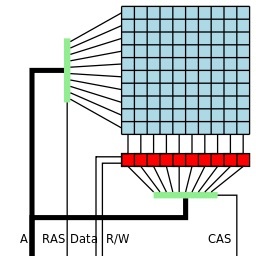
\includegraphics[width=0.5\linewidth]{images/chapter_9/DRAM.jpg}
	\caption{High Level Illustration of DRAM Organization (Source: Wikipedia:Row Hammer)}\label{fig:dram_svg}
\end{figure}

\subsection{Double-sided Rowhammer}\label{subsec:double_sided_rowhammer}
DRAM is the most common type of volatile memory. It is slow, dense and cheap
relatively to SRAM\@. Every bit of RAM is stored in a single capacitor.

The attack~\cite{rowhammer} utilizes the physical structure of RAM chips in
order to induce faults: Due to parasitic leakage in DRAM capacitors, if enough
consecutive reads are performed on the immediately adjacent rows eventually a
bit will flip in the target row.

\subsubsection{The challenge of CPU caching}\label{subsubsec:the_challenge_of_cpu_caching}
The CPU cache prevents the same memory address to be read consecutively from
main memory, for performance reasons. To circumvent this limitation, several
techniques can be employed:
\begin{enumerate}
	\item Intel CPUs provide non-temporal read/write opcodes -- special
	instructions that read from memory and don't get cached.
	\item The special \texttt{clflush} instruction can be used to explicitly
	flush the cache after each read operation (privileged operation).
	\item Finally, cache-population algorithms had been extensively studied and
	reverse-engineered, so it is possible to arrange for \emph{arbitrary} cache
	misses.
\end{enumerate}

\subsection{Countermeasures}\label{subsec:countermeasures}
\paragraph{Refresh-rate increase:} In order to overcome parasitic leakage, DRAM
chips already have a mechanism in place to read and then re-write the values
stored in each row periodically. One method of overcoming Rowhammer could be to
significantly increase the refresh-rate of the chip. This obviously results in
both performance degradation and increased power consumption.

\paragraph{ECC-RAM:} High-end DRAM chips (typically meant for data center
environments) contain error-correction coding (ECC) logic which can typically
\emph{correct} one erroneous bit and \emph{detect} two (at which point it will
crash the program/system). Those chips are immune to the basic form of Rowhammer
described above, but as discussed later, are not bullet-proof.

\subsection{Rowhammer variations}\label{subsec:rowhammer_variations}
\subsubsection{Flip Feng-Shui}\label{subsubsec:flip_feng_shui}
\paragraph{Page de-duplication:} On modern systems, typically much memory is
shared among many processes running on the system. This is even more true of
virtualized environments where the guest and the host, for example, could run
the same OS\@. A common optimization is for the system to detect and
de-duplicate pages containing the same data, thus freeing up memory.
\paragraph{Rowhammer + page de-duplication:}
In a paper~\cite{ffs} researchers from VUA demonstrated how they can utilize
page-deduplication in a virtualized environment to weaken cryptographic keys,
resulting in unauthorized access via OpenSSH, and breach of trust via forging
GPG signatures. The attack relies on the fact that the the attacker can
\emph{read} a de-duplicated page as much as they want. The attacker has to wait
(or arrange) for a page containing sensitive information to be de-duped, then
hammer on it until a bit in the key flips, making it much easier to factor.
\begin{figure}[!ht]
	\centering
	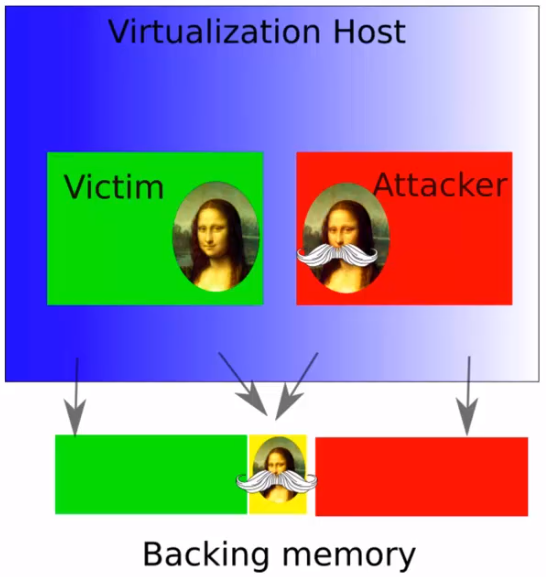
\includegraphics[width=0.5\linewidth]{images/chapter_9/flip_feng_shui.PNG}
	\caption{The attacker maps the same page as the victim, then utilizes rowhammer to change the victim's memory without causing page duplication.}
	\label{fig:flip_feng_shui}
\end{figure}

\subsubsection{ECCPloit}\label{subsubsec:eccploit}
In another paper~\cite{eccploit} researchers from VUA showed how they can use
Rowhammer to quickly flip \emph{enough} (typically three) bits on an ECC-RAM
chip that error correction will not be able to detect it, thus defeating the ECC
mitigation. The attack relies on the fact that error-correction takes time to
compute, and this gives the attacker a window of opportunity.

\subsection{Rowhammer-based attacks}
\subsubsection{RAMBleed}
We will describe here Rowhammer based attack called RAMbleed which was presented in ~\cite{rambleed_paper}. While Rowhammer breaks data integrity, RAMBleed breaks also data confidentiality by allow the attacker read unauthorized memory areas. RAMBleed attack was implementes against OpenSSH server allowing the attacker read RSA secret private keys. 

\begin{figure}[!ht]
	\centering
	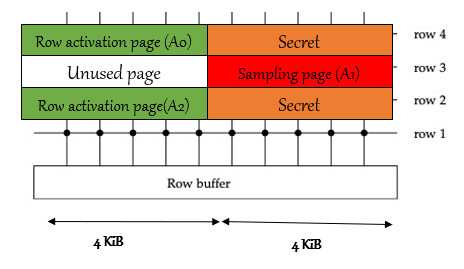
\includegraphics[width=0.7\linewidth]{images/chapter_9/rambleed_memory_layout.png}
	\caption{RAMBleed memory layout}
	\label{fig:rambleed_memory_layout}
\end{figure}
In order to perform this attack, the attacker need to get to spesific memory layout, as describe in \Cref{fig:rambleed_memory_layout}. The attacker own A0, A1 and A2 block. Then attacker force OpenSSH server to put its private RSA key in oranges blocks by exploting linux buddy allocator which works in deterministic way. Then the attacker repeatedly accessing A0 and A2 blocks - this will access orange blocks 
as well because when DRAM access a part of the row, it access the whole row as well. This will hammer the red block and cause bit flips over there. The attacker can then read the red block- because he own it, and gets the RSA secret key.

The performence from this paper shows accuracy of 82\% when reading OpenSSH host key. Reading the victim’s secret in 0.31 bits/seconds.

Suggested mitigations may be memory encryption, flushing keys from memory, probabilistic memory allocator and Hardware mitigations such as targeted row refresh and increasing refresh intervals.



\section{Related Work} \label{sec:RelatedWork}

Additional related work on the topic of fault attacks includes:

\begin{itemize}

	\item \textbf{DVFS} - Dynamic Voltage and Frequency Scaling 
	attacks make use of voltage and frequency combinations
	which are considered unstable.

	\begin{itemize}

		\item \textbf{CLKScrew} - a paper by 
		Tang et al that describes a technique that takes advantage of security vulnerabilities
		caused by the constant strive to improve energy efficiency, more specifically energy management
		mechanisms used in state-of-the-art mobile SoCs.

		\item \textbf{VoltJockey} - a paper by Qiu et al that describes a hardware fault-based attack on 
		the TrustZone - a security approach deployed in ARM processors. This attack
		uses software-controlled voltage manipulation. It is demonstrated on an ARM-based
		multi-core processor and manages to acquire an AES key protected by TrustZone.
		
		\item \textbf{Plundervolt} - a paper by Murdock et al, the first one that describes 
		the use of voltage scaling for corruption of integrity and confidentiality
		of Intel SGX enclaved computations. The authors demonstrate full key recovery PoC attacks
		against RSA-CRT and AES-NI.
		
		
	\end{itemize}

	\item \textbf{Speculative Fault Attacks} - Such attacks make use of the behavior of modern
	processors and their attempt to predict and speculate the next instructions to be executed
	for maximum performance. CPUs will try to execute instructions ahead of time.

	\begin{itemize}

		\item \textbf{Spectre - Exploting Speculative Execution} - a paper by Kocher et al that describes
		a speculative fault attack that involves inducing a victim to speculatively perform operations
		that would not occur during correct program execution and which leak the victim's confidential
		information via a side-channel to the adversary.
		
	\end{itemize}

\end{itemize}